\documentclass{beamer}
\usepackage[utf8]{inputenc}

\usetheme{Madrid}
\usecolortheme{default}
\usepackage{amsmath,amssymb,amsfonts,amsthm}
\usepackage{txfonts}
\usepackage{tkz-euclide}
\usepackage{listings}
\usepackage{adjustbox}
\usepackage{array}
\usepackage{tabularx}
\usepackage{gvv}
\usepackage{lmodern}
\usepackage{circuitikz}
\usepackage{tikz}
\usepackage{graphicx}
\usepackage{mathtools}
\setbeamertemplate{page number in head/foot}[totalframenumber]

\usepackage{tcolorbox}
\tcbuselibrary{minted,breakable,xparse,skins}



\definecolor{bg}{gray}{0.95}
\DeclareTCBListing{mintedbox}{O{}m!O{}}{%
  breakable=true,
  listing engine=minted,
  listing only,
  minted language=#2,
  minted style=default,
  minted options={%
    linenos,
    gobble=0,
    breaklines=true,
    breakafter=,,
    fontsize=\small,
    numbersep=8pt,
    #1},
  boxsep=0pt,
  left skip=0pt,
  right skip=0pt,
  left=25pt,
  right=0pt,
  top=3pt,
  bottom=3pt,
  arc=5pt,
  leftrule=0pt,
  rightrule=0pt,
  bottomrule=2pt,
  toprule=2pt,
  colback=bg,
  colframe=orange!70,
  enhanced,
  overlay={%
    \begin{tcbclipinterior}
    \fill[orange!20!white] (frame.south west) rectangle ([xshift=20pt]frame.north west);
    \end{tcbclipinterior}},
  #3,
}
\lstset{
    language=C,
    basicstyle=\ttfamily\small,
    keywordstyle=\color{blue},
    stringstyle=\color{orange},
    commentstyle=\color{green!60!black},
    numbers=left,
    numberstyle=\tiny\color{gray},
    breaklines=true,
    showstringspaces=false,
}
%This block of code defines the information to appear in the
%Title page
\title %optional
{2.5.25}
%\subtitle{A short story}

\author % (optional)
{Vaishnavi - EE25BTECH11059}



\begin{document}


\frame{\titlepage}
\begin{frame}{Question}
Let $\mathbb{R}^3$ denote the three-dimensional space. 
Take two points $P = (1,2,3)$ and $Q = (4,2,7)$. 
Let $\text{dist}(X,Y)$ denote the distance between two points $X$ and $Y$ in $\mathbb{R}^3$. 

Let
\[
S = \{X \in \mathbb{R}^3 : (\text{dist}(X,P))^2 - (\text{dist}(X,Q))^2 = 50 \}
\]
and
\[
T = \{Y \in \mathbb{R}^3 : (\text{dist}(Y,Q))^2 - (\text{dist}(Y,P))^2 = 50 \}.
\]

Then which of the following statements are TRUE? 
 

\end{frame}
\begin{frame}{allowframebreaks}
\frametitle{Solution}
\begin{table}[H]    
  \centering
  \begin{tabular}{|c|c|}
\hline
\textbf{Variable} & \textbf{Value} \\
\hline
$A$ & $(0,-\frac{3}{2})$ \\
\hline
$m$ & $\frac{1}{2}$ \\
\hline
\end{tabular}
  \caption{Variables Used}
  \label{tab:1.10.25}
\end{table}

\end{frame}


\begin{frame}{Solution}
\begin{align}
                                     \vec{P}= \myvec{
                                             1
                                              \\
                                              2
                                               \\
                                               3
                                              }
\end{align}
\begin{align}
                                     \vec{Q}= \myvec{
                                             4
                                              \\
                                              2
                                               \\
                                               7
                                              }
\end{align}
\begin{align}
 \text{dist}(X,P))^2 - (\text{dist}(X,Q))^2 = 50 \\
 (\|\vec{X}-\vec{P}\|_2)^2- (\|\vec{X}-\vec{Q}\|_2)^2=50
\end{align}

\end{frame}

\begin{frame}{solution}
\begin{align}
\vec{X^T}\vec{X}-2\vec{P^T}\vec{X}+\vec{P^T}\vec{P}-\vec{X^T}\vec{X}
+2\vec{Q^T}\vec{X}-\vec{Q^T}\vec{Q}=50\\
2(\vec{Q^T}-\vec{P^T})\vec{X}+\vec{P^T}\vec{P}-\vec{Q^T}\vec{Q}=50
\end{align}
(0.6)is the eq of plane S
\begin{align}
\text{dist}(Y,Q))^2 - (\text{dist}(Y,P))^2 = 50\\
 (\|\vec{Y}-\vec{Q}\|_2)^2- (\|\vec{Y}-\vec{P}\|_2)^2=50
\end{align}
\end{frame}
\begin{frame}{Solution}
\begin{align}
\vec{Y^T}\vec{Y}-2\vec{Q^T}\vec{Y}+\vec{Q^T}\vec{Q}-\vec{Y^T}\vec{Y}
+2\vec{P^T}\vec{Y}-\vec{P^T}\vec{P}=50\\
2(\vec{P^T}-\vec{Q^T})\vec{Y}+\vec{Q^T}\vec{Q}-\vec{P^T}\vec{P}=50
\end{align}
(0.10) is the eq of plane T\\
S And T are parallel planes\\


\end{frame}
\begin{frame}{Solution}
S is an infinite plane. In any plane one can choose three non collinear points whose triangle has unit area.Therefore a) is correct 
\\
\\
let eq of T be $\vec{n^T}\vec{X}=c$\\
let $\vec{A},\vec{B}$ be two points on T\\
\begin{align}
    \vec{n^T}\vec{A}=c\\
    \vec{n^T}\vec{B}=c
\end{align}
\end{frame}
\begin{frame}{Solution}
any point on line AB can be written as
\begin{align}
    \vec{C}=(1-k)\vec{A}+k\vec{B}\\
    \vec{n^T}[(1-k)\vec{A}+k\vec{B}]
   = \vec{n^T}\vec{A}+k[\vec{n^T}\vec{B}-\vec{n^T}\vec{A}]
   =c\\
   \vec{n^T}\vec{C}=c
\end{align}
Hence C lies on T \\
Therefore b) is correct\\
\end{frame}
\begin{frame}{Solution}
distance between S and T=$\frac{\lvert c_1 - c_2 \rvert}{|n|}
=10$\\
let $\vec{A},\vec{B}$ lie on S and $\vec{A'},\vec{B'}$
where 
\begin{align}
 \|\vec{A}-\vec{B}\|_2=\|\vec{A'}-\vec{B'}\|_2=d(say)\\
 2(d+10)=48\\
 d=14
\end{align}

There are infinitely many ways to pick two points in plane 
S that are 14 units apart (because the plane is infinite).\\
Therefore c) is correct
\end{frame}
\begin{frame}{Solution}
The distance between the planes $S$ and $T$ is $10$. A square with perimeter $48$ has side length $12$.  
If two opposite vertices lie on $S$ and the other two on $T$, then each side of the square must connect the two planes.  
Since the vertical separation is $10$, and the side is $12$, the square can be tilted so that part of the side length is vertical ($10$ units) and the rest is horizontal: ($\sqrt{12^2 - 10^2} = \sqrt{44}$ units)


Hence d) is correct
\end{frame}
\begin{frame}{Graph}
   Refer to Figure

\begin{figure}[H]
\begin{center}
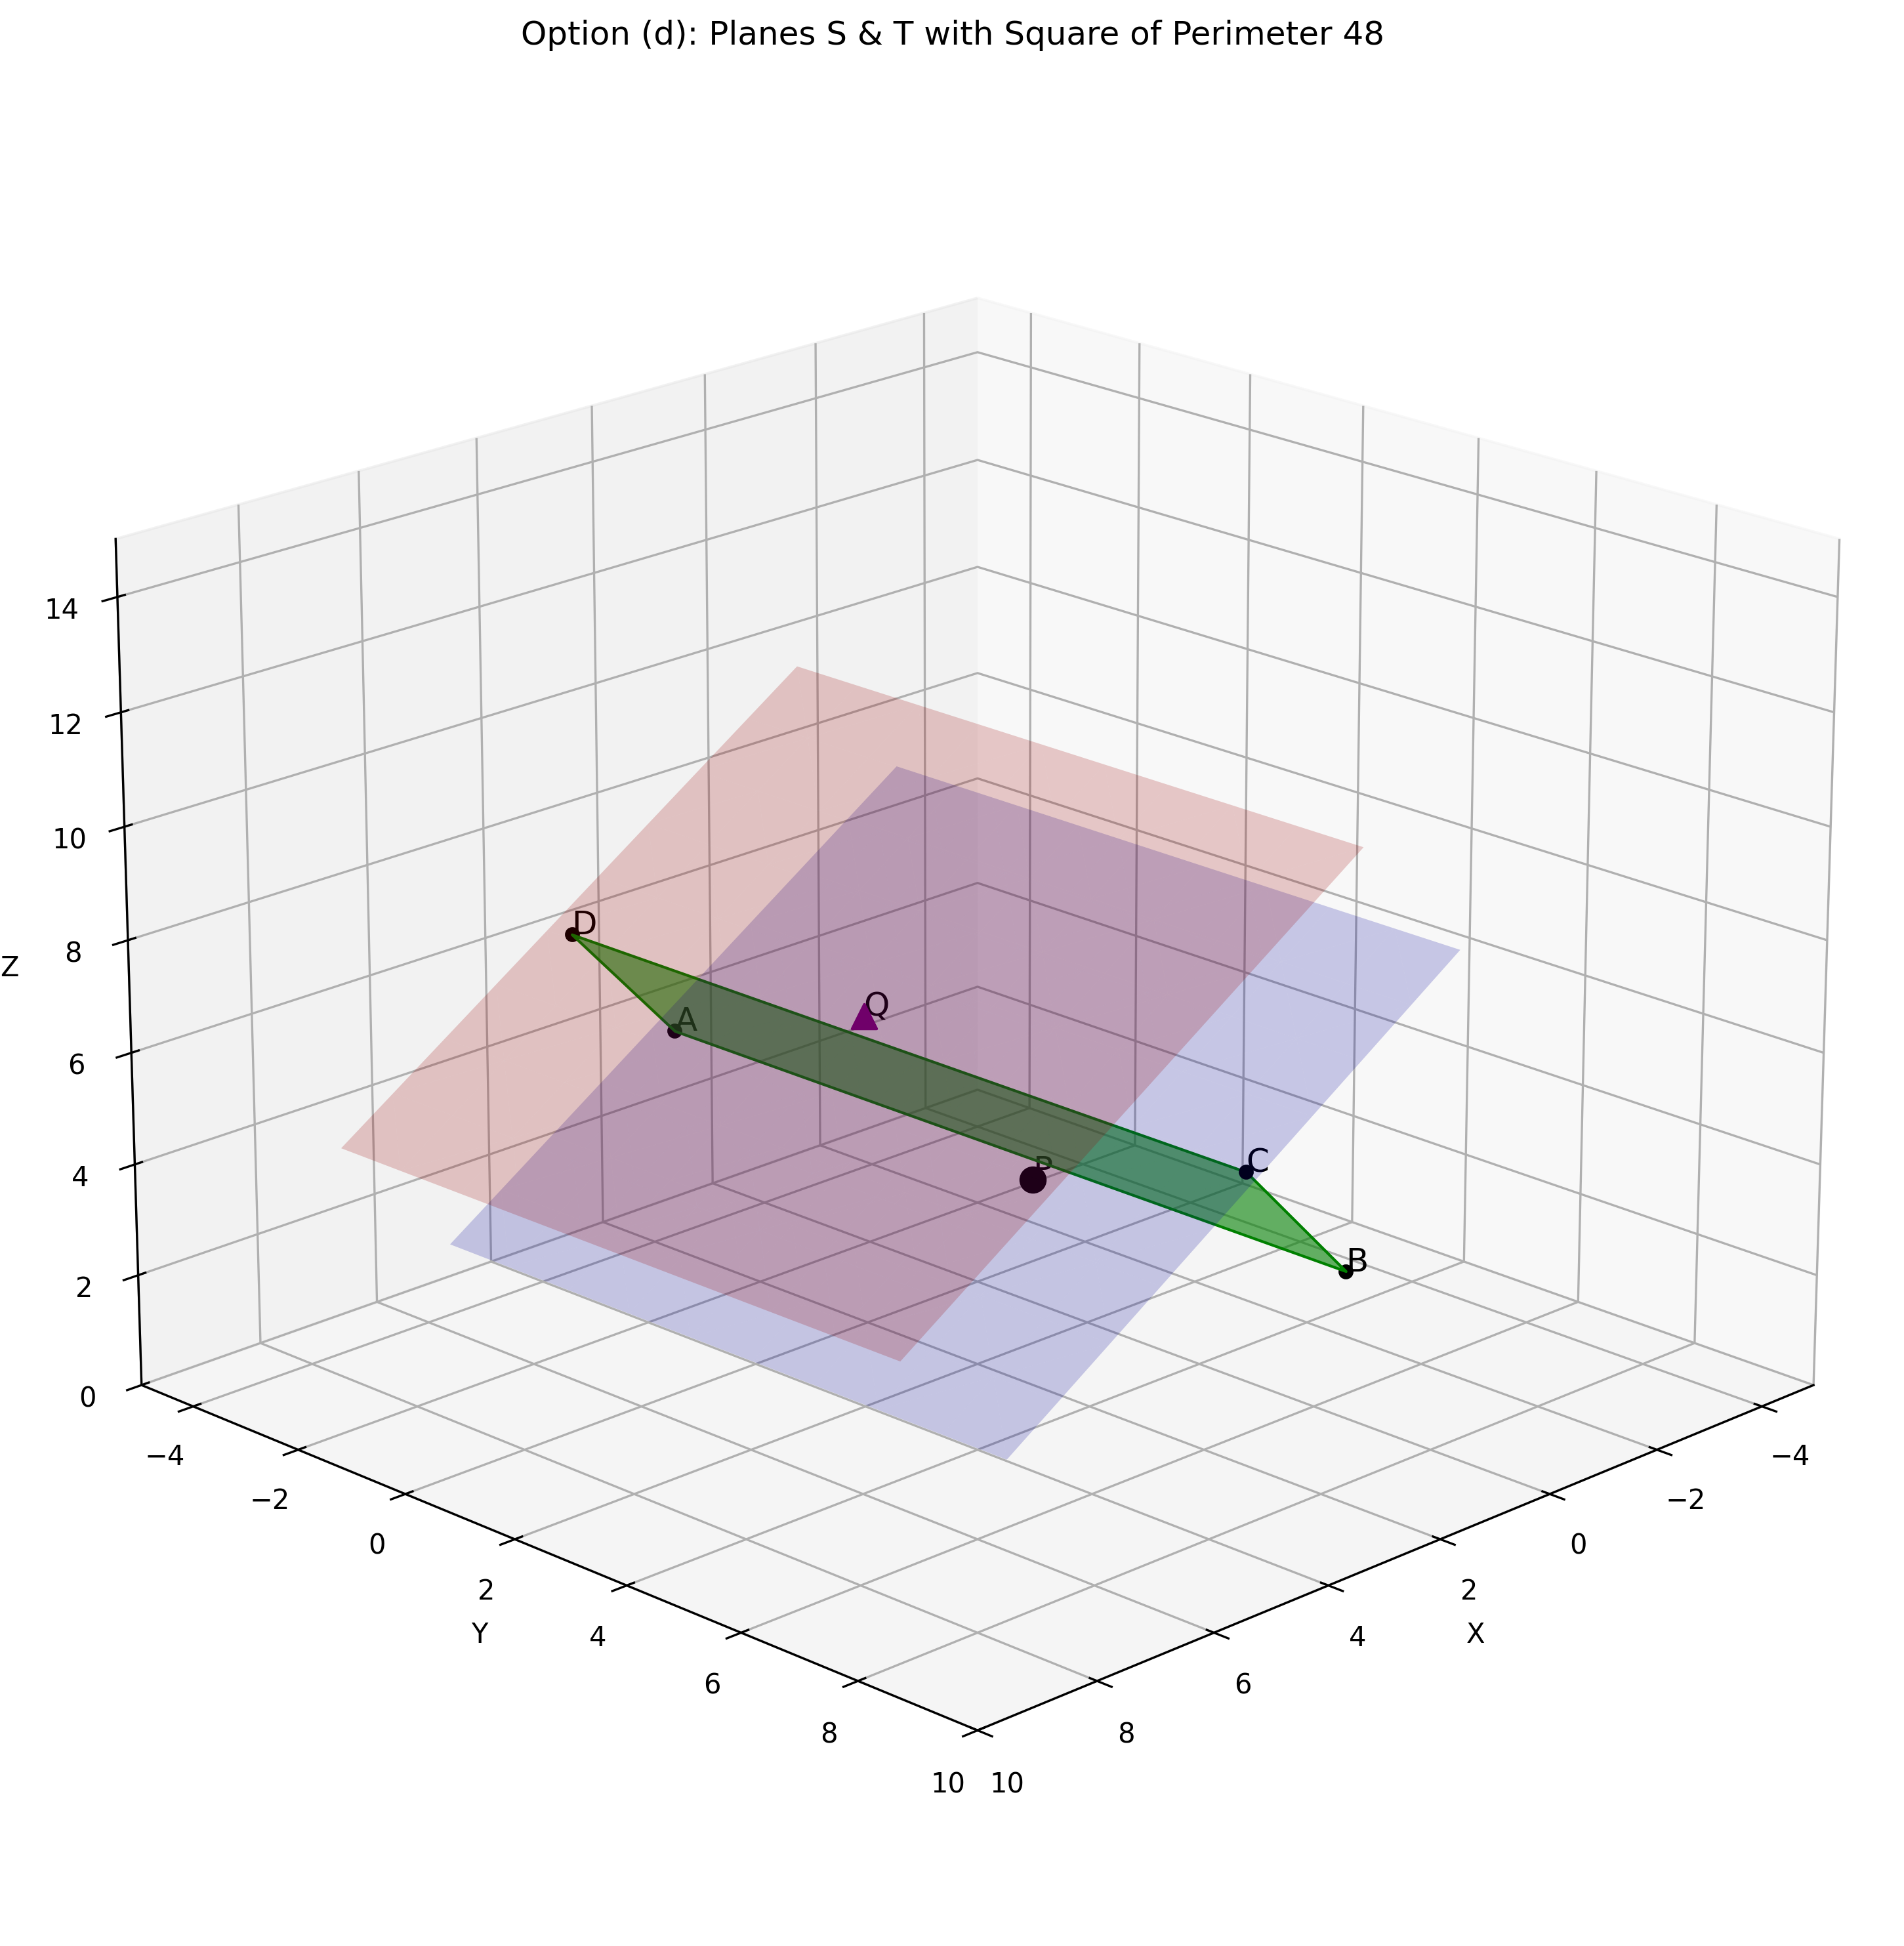
\includegraphics[width=0.6\columnwidth]{../figs/graph5a.png}
\end{center}
\caption{}
\label{fig:Fig}
\end{figure}  
\end{frame}



\begin{frame}[fragile]
    \frametitle{Python Code}
    \begin{lstlisting}
import matplotlib.pyplot as plt
import numpy as np

# Define vectors
a = np.array([2, -1, -2])
b = np.array([7, 2, -3])
b1 = np.array([4, -2, -4])
b2 = np.array([3, 4, 1])

# Function to draw vectors
def draw_vector(ax, start, vec, color, label):
    ax.quiver(*start, *vec, color=color, label=label, arrow_length_ratio=0.1)

# Create 3D plot
fig = plt.figure(figsize=(10,8))
ax = fig.add_subplot(111, projection='3d')
\end{lstlisting}
\end{frame}

\begin{frame}[fragile]
    \frametitle{Python Code}

    \begin{lstlisting}
# Draw from origin
origin = np.array([0,0,0])
draw_vector(ax, origin, a, 'blue', 'a')
draw_vector(ax, origin, b, 'red', 'b')
draw_vector(ax, origin, b1, 'green', 'b1 (parallel to a)')
draw_vector(ax, origin, b2, 'purple', 'b2 (perpendicular to a)')

# Show b as b1 + b2 (parallelogram completion)
draw_vector(ax, b1, b2, 'orange', 'b1 + b2 = b')

# Labels and title
ax.set_xlabel('X', fontsize=12)
ax.set_ylabel('Y', fontsize=12)
ax.set_zlabel('Z', fontsize=12)
ax.set_title("3D Representation of Vectors a, b, b1, and b2", fontsize=14)
ax.legend()


    \end{lstlisting}
\end{frame}

\begin{frame}[fragile]
    \frametitle{Python Code}

    \begin{lstlisting}
# Grid and aspect ratio
ax.grid(True)
ax.set_box_aspect([1,1,1])

# Axis limits
ax.set_xlim(0,8)
ax.set_ylim(-3,6)
ax.set_zlim(-5,2)

# Save figure
plt.savefig("Graph3.png", dpi=300, bbox_inches='tight')
plt.show()



  \end{lstlisting}
\end{frame}

\begin{frame}[fragile]
\frametitle{C Code}
\begin{lstlisting}
#include <stdio.h>
#include <math.h>

#define MAX_POINTS 10000
#define STEP 1.0
#define TOL 0.5  // tolerance
#define SIDE_LENGTH 12.0

typedef struct {
    double x, y, z;
} Point;

double dist2(Point a, Point b) {
    return (a.x - b.x)*(a.x - b.x) +
           (a.y - b.y)*(a.y - b.y) +
           (a.z - b.z)*(a.z - b.z);
}

    \end{lstlisting}

\end{frame}

\begin{frame}[fragile]
\frametitle{C Code}
\begin{lstlisting}
  void solve_vectors() {
    Point P = {1, 2, 3};
    Point Q = {4, 2, 7};

    Point S[MAX_POINTS];
    Point T[MAX_POINTS];
    int s_count = 0, t_count = 0;

    for (double x = -10; x <= 10; x += STEP) {
        for (double y = -10; y <= 10; y += STEP) {
            for (double z = -10; z <= 10; z += STEP) {
                Point A = {x, y, z};
                double lhs = dist2(A, P);
                double rhs = dist2(A, Q);
                double d = lhs - rhs;
\end{lstlisting}
\end{frame}
\begin{frame}[fragile]
\frametitle{C Code}
\begin{lstlisting}
 if (fabs(d - 50.0) < TOL && s_count < MAX_POINTS) {
                    S[s_count++] = A;
                } else if (fabs(-d - 50.0) < TOL && t_count < MAX_POINTS) {
                    T[t_count++] = A;
                }
            }
        }
    }

    printf("Found %d points on Set S and %d points on Set T.\n", s_count, t_count);

    for (int i = 0; i < s_count; i++) {
        for (int j = 0; j < t_count; j++) {
            double d = sqrt(dist2(S[i], T[j]));
            if (fabs(d - SIDE_LENGTH) < TOL) {
                printf("Found square side length %.2f\n", d);
                printf("S-point: (%.2f, %.2f, %.2f)\n", S[i].x, S[i].y, S[i].z);
                printf("T-point: (%.2f, %.2f, %.2f)\n", T[j].x, T[j].y, T[j].z);
                return;
            }
        }
    }
    printf("No square found.\n");
}
\end{lstlisting}
\end{frame}


\begin{frame}[fragile]
\frametitle{Python and C Code}

\begin{lstlisting}
iimport ctypes

# Load the shared library
lib = ctypes.CDLL('./code.so')

# Call the function
lib.solve_vectors()

\end{lstlisting}

\end{frame}

 





\end{document}